\section*{rep-10}
The code in figure \ref{fig:rep10} generates the plot for the first subtask of this exercise. It generates a plot, showing the \textit{\#pkts/hour}. The only difference to the other subtasks is in line 6 of this code snippet. Here the parameter 3 describes the column index of the data we want to plot. The indices for subtask 2-4 can be seen in table \ref{tab:indices}.
\begin{table}[H]
\center
\begin{tabular}{lr}
\toprule
index & feature name \\
\midrule
2 & \#bytes / hour (daily avg.) \\
4 & \#uIPs / hour (daily avg.) \\
5 & \#uIPd / hour (daily avg.) \\
\bottomrule
\end{tabular}
\caption{Indices for the several dataset features}
\label{tab:indices}
\end{table}
\begin{figure}[H]
\lstinputlisting{./chapters/matlab/team16_ex3_rep10_1.m}
\caption{Matlab code for first subtask of rep-10}
\label{fig:rep10}
\end{figure}

In addition a function was implemented, for plotting a graph, which also deals with the epoch to datenum format conversion. The exact implementation of this function is listed in figure \ref{fig:plotDarkNetData}.

\begin{figure}[H]
\lstinputlisting{./chapters/matlab/plotDarknetData.m}
\caption{Matlab code for the 'plotDarknetData' function}
\label{fig:plotDarkNetData}
\end{figure}

For the normalization we simply loaded every feature set in a separate feature vector and devided it by the vectors max value. In figure \ref{fig:normalization} the normalization is demonstrated on the first feature \(\#pkts/hour\). The smoothing, as described in the exercise description, was implemented in the matlab function 'smoothLine'.

\begin{figure}[H]
\lstinputlisting{./chapters/matlab/team16_ex3_rep10_5_normalization.m}
\caption{Matlab code for the normalization}
\label{fig:normalization}
\end{figure}


\subsection*{Results}
\begin{figure}[H]
\center
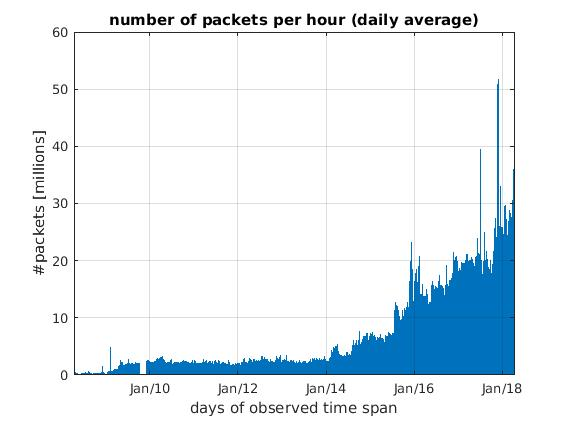
\includegraphics[width=.7\textwidth]{./chapters/plots/rep10_1.jpg}\\
\caption{Results of rep10-1}
\end{figure}
\begin{figure}[H]
\center
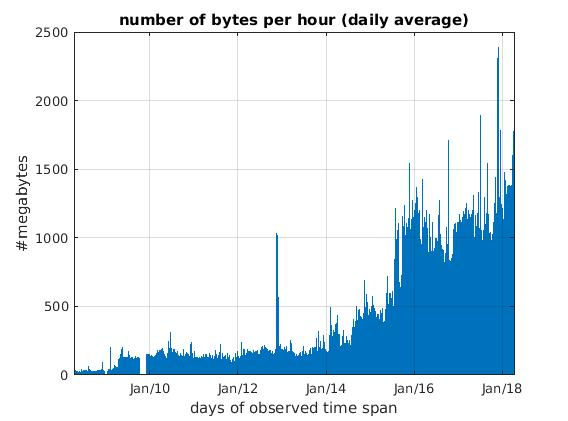
\includegraphics[width=.7\textwidth]{./chapters/plots/rep10_2.jpg}\\
\caption{Results of rep10-2}
\end{figure}
\begin{figure}[H]
\center
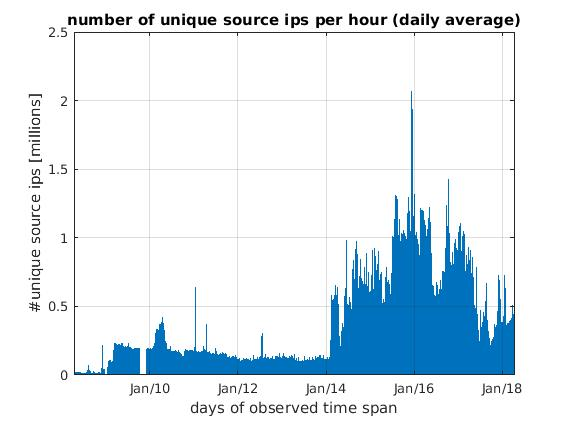
\includegraphics[width=.7\textwidth]{./chapters/plots/rep10_3.jpg}\\
\caption{Results of rep10-3}
\end{figure}
\begin{figure}[H]
\center
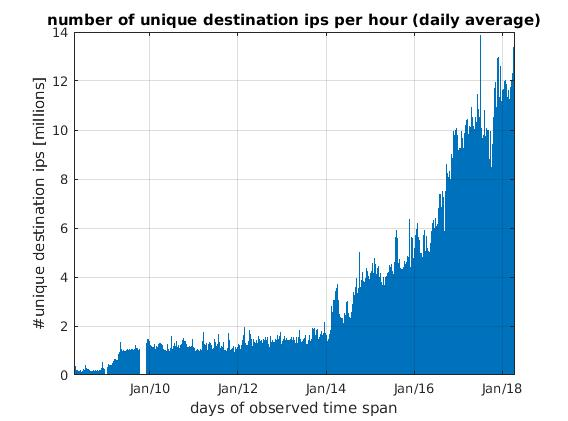
\includegraphics[width=.7\textwidth]{./chapters/plots/rep10_4.jpg}\\
\caption{Results of rep10-4}
\end{figure}

\section*{rep-11}
For this task, the correlation matrix was calculated by executing the matlab code of figure \ref{fig:correlation}
\begin{figure}[H]
\lstinputlisting{./chapters/matlab/team16_ex3_rep11.m}
\caption{Matlab code for the normalization}
\label{fig:correlation}
\end{figure}
The resulting correlation matrix (figure \ref{matrix:correlation}) shows us, that the \text{\#unique source IP addresses per hour} show the lowest correlation values, especially with the \textit{\#unique destination IP addresses per hour}. Especially for the unique IP sources, it is noticeable, that there is a drop after Jan/16. This drop does not correlate to the other features, which means, a lot of traffic is generated by one host, which accesses a lot of different source IPs. This can be a sign of horizontal scanning!

\begin{figure}[H]
\center
$
\begin{bmatrix}
1.000 &  0.965 &  0.720 &  0.934 \\
0.965 &  1.000 &  0.610 &  0.973 \\
0.720 &  0.610 &  1.000 &  0.589 \\
0.934 &  0.973 &  0.589 &  1.000
\end{bmatrix}
$
\caption{correlation matrix of the dataset containing the values for all 4 features}
\label{matrix:correlation}
\end{figure}

\section*{rep-12}
In order to find out, if there are more sources sending data to the darkspace, than addresses receiving data from it, the ratio between the unique source and destination IPs is calculated, as shown in figure \ref{fig:ratio_source_destination_ip}.

\begin{figure}[H]
\lstinputlisting{./chapters/matlab/team16_ex3_rep12_less.m}
\caption{Matlab code for calculating the ratio between the average unique source addresses and the average unique destination addresses per hour.}
\label{fig:ratio_source_destination_ip}
\end{figure}

The ratio between source and destination IPs is $9.31$. This means, that there are approximately 10 times more addresses receiving data from the darspace. This result was expected, as \textit{rep-11} already showed, that there is a horizontal scan going on.

\section*{rep-13}
To find the peak of the '\#uIPs/hour (daily avg.)', the first column was converted to datenum format before retrieving the maximum value of the '\#uIPs/hour (daily avg.)' column. The \textit{max} function retrieves the maximum value and it's index. This index we use to retrieve the Date of this peak. This three steps are listed in figure \ref{fig:find_peak}.

\begin{figure}[H]
\lstinputlisting{./chapters/matlab/team16_ex3_rep13_less.m}
\caption{Matlab snipped for finding the peak of '\#uIPs/hour (daily avg.)'}
\label{fig:find_peak}
\end{figure}

This commands lead to the finding, that the peak occured on the 15th of December 2015. As the neighbor values (14th and 16th of December) are significantly smaller, the peak lasted only for one day.

\section*{rep-14}
Table \ref{tab:stat_jun2017_gen} shows the statistical values for the \textit{Jun2017\_gen.csv} file and table \ref{tab:stat_jun2017_global} shows statistical values for the same time periode, but the data was extracted from the \textit{global\_last10years.csv} file. 
\begin{table}[H]
\center
\begin{tabular}{lrrrr}
\toprule
feature & total sum & mean & median & std. deviation \\
\midrule
\#pkts/hour & 6 922.229  &   9.695  &    9.937  &   1.443 \\
\#bytes/hour & 207.103  &   0.290   &   0.241  &   0.098 \\
\#uIPs/hour  & 13 157.867  &  18.428  &   18.511 &    4.329 \\
\#uIPd/hour  & 719 606.146 &  1 007.852 &   993.364 &  237.632 \\
\bottomrule
\end{tabular}
\caption{Statistics of June 2017 from Jun2017\_gen.csv (in millions)}
\label{tab:stat_jun2017_gen}
\end{table}

\begin{table}[H]
\center
\begin{tabular}{lrrrr}
\toprule
feature & total sum & mean & median & std. deviation \\
\midrule
\#pkts/hour  &    291.275  &      9.709  &      9.996   &    1.169 \\
\#bytes/hour &      8.700  &      0.290  &      0.254   &    0.076 \\
\#uIPs/hour  & 30 268.997  &  1 008.967  &  1 008.526   &  101.158\\
\#uIPd/hour  &    553.823  &     18.461  &     19.124   &    3.080 \\
\bottomrule
\end{tabular}
\caption{Statistics of June 2017 from global\_last10years.csv (in millions)}
\label{tab:stat_jun2017_global}
\end{table}

\section*{rep-15}
Comparing table \ref{tab:stat_jun2017_gen} and \ref{tab:stat_jun2017_global} leads to the conclusion, that some values do coincide, but not all. Especially for the \textit{total sum} column, there are big differences. The problem is, that in the first table the averages for every hour are summed up and compared to the averaged value of the second table, therefore it is not surprising, that the \textit{total sum} values of table \ref{tab:stat_jun2017_global} are significantly smaller.
There are also differences, when it comes to '\#uIPs/hour' and '\#uIPd/hour'. The problem here is, that in the table \ref{tab:stat_jun2017_gen}, the same IP occuring every hour of the same day, is counted as a unique IP, where as in table \ref{tab:stat_jun2017_global} this IP address would be counted for the whole day as \textbf{one} unique IP address.
Mean, median and standard deviation values for '\#pkts/hour' and '\#bytes/hour' are not sensitive to those problems, therefore they do coincide in both tables.

\section*{rep-16}

\section*{rep-17}

\section*{rep-18}

% \section*{rep-19} OPTIONAL

% \section*{rep-20} OPTIONAL

\section*{rep-21}

\section*{rep-22}

\section*{rep-23}

